\section{Stakeholders}
  \begin{figure}
    \centering
    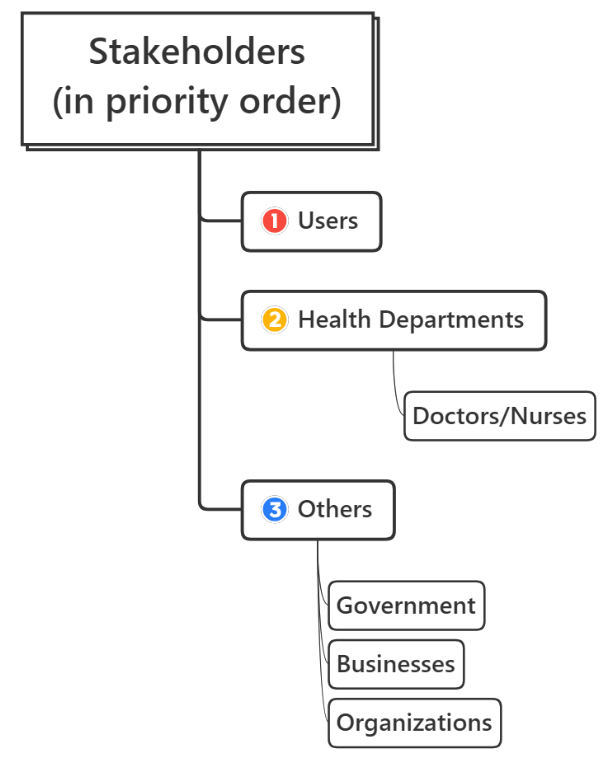
\includegraphics[width=12cm]{stakeholders.png}    
    \caption{Stakeholders}
  \end{figure}

  \subsection{Users}
    \par It is obvious that this app is designed for everyone around the world. All you need is a smartphone or a wearable device to install the app. At the time when the pandemic seems to be out of control, this app is a considerable solution that helps users gain more understanding of their health conditions. It cannot be denied that when the scene is extremely dangerous, social distancing is one of the best solutions to prevent the virus from spreading. However, there are some situations that people must go outside such as grocery shopping or medical appointments \parencite{Stake1}. It is impossible to lock yourself inside your house 24/7. This app will help to track all other people that the user has been in contact with when they were outside. Although the number of people might be modest thanks to social distancing, prevention is still compulsory. Moreover, there are specific jobs that people cannot work from home. People may be working in public services, in retail, in vital parts of the manufacturing sector or for the governments \parencite{Stake2}. These paramount jobs cannot be converted instantly into homeworking. Therefore, there will still be several people heading out for works facing a high risk of infection. This app will support those people by storing the data of everyone they have met at the workplace or on the way to work.
    \par During  application  development,  data  security  is  always  the  top  priority. There are lots of users who do not want to install the application if it has access to their location 24/7. Therefore, the application is designed perfectly to protect their privacy. All information and data will be stored locally and uploaded to theserver only with the permission of the user. Although the government owns the servers, no one will have access to the data in servers. The most important feature is that each user has their own unique ID and this ID is regenerate after a short period of time. With  this  feature,  data  security  is  absolutely  guaranteed.  Besides  contact  tracing, users will benefit greatly from this application. They can easily find official news or detailed information aboutthe disease situationin the application. The application also gathers support packages thatare offeredby trustworthy organizations out there. It is difficult fortheuser to look up for those packages on the internet because there are countless of them and they can not know which one is legit. The application will supportthe  user  in  finding  packages  that  fit  their  needs  and  backgrounds.These convenient features will attract more users including the fastidious ones.

  \subsection{Doctors/Nurses}
    \par Doctors and nurses probably benefit a lot from this app. The more we prevent the virus from spreading, the less the pressure on them. In countries which are facing the pandemic like Italy, doctors have to make heartbreaking decisions about who receives the treatment and who is abandoned \parencite{Stake3}. Furthermore, because of the sudden rise in the number of infected cases, there is not enough equipment for health workers \parencite{Stake4}. Consequently, many of them are risking their lives curing patients. Healthcare workers are influential in the war with pandemics and protecting them should be the number one priority. If they are infected, they must be isolated for at least 14 days, which will deplete the already exhausted workforce \parencite{Stake5}. By reducing the number of cases, doctors will be in contact with fewer infected patients. Finally, the situation of the pandemic is serious does not mean that we neglect patients with other sicknesses.
    \par This  application  also  needs  the  cooperation  of  the  Health  Organization  or Health Department to obtain all the information about the current pandemic (namely symptoms,  how  it  spreads,  how  to  protect  yourself,  etc.).  With  these  data,  the application  can  adapt  and  use  the  most  effective  tracking  method. Reliable and necessary information about the disease will be provided to usersin various forms. The Health Department is also responsible for the Q\&A form that is given to users. They will be the ones who understand best what questionsare needed in the formand ways to analyze user answersin order toassess the rate of infection.

  \subsection{Governments/Health Departments/Health Organizations}
    \par It cannot be denied that governments play an important role in stopping the spread of pandemics. They are the frontline and their decisions highly influencing the fight against the epidemics. The governments have adopted some regulations like social  distancing  to  protect  and  support  their  people.    It  is  the  governments’ responsibility to track the virus and put an end to it. With this app, they can easily find  out  who  the  infected  patient  has  been  in  contact  with  instead  of  inquiring him/her.  The  results  came  out  from  investigating  infected  patients  might  be inaccurate due to the unstable health condition of them. Another  problem that the governments and health departments are facing during the pandemic outbreak is the shortage  of  hospital  beds.  For  instance,  in  the  US,  many  hospitals  have  become overloaded \cite{Stake6}.  Based  on  overseas  experience,  about  one-fifth  of  people  infected with COVID-19 need hospital care and 5\% will need intensive care because of their critical  health  status \cite{Stake3}.  Therefore,  if  the  coronavirus  keeps  spreading  with  the ongoing rate, the number of infected patients will exceed the number of available beds soon. In response, the governmentshavebuilt more field hospitalswhich only cure COVID-19 patients. As proof, a dedicated coronavirus field hospital is being built in Canberra which could cost more than \$23 million \cite{Stake7}. This application helps to reduce the number of infected cases also means that governments can save a lot of money.

    \par The governments will administer the servers for this application.When a useris diagnosed as infected, he/she will voluntarily upload the contact logging list to the servers and other users will download that list to the mobile devices for comparison. Although  the  servers  are  under  the  control  of  the  governments,  the  list  is  not accessible for them to ensure user privacy. The governments are also in charge of enact laws to make businesses and people follow the government–business–user cooperation model. Last but not least, the government must support to bring the app  to a wide range of users. Themoreusers, the more this applicationcan put into actionits full potential.

  \subsection{Businesses}
    \par Not only a health concern, COVID-19 is seriously impacting business and the economy. It cannot be denied that this pandemic is affecting many aspects of the economy. According to data from the Australian Bureau of Statistics (ABS), approximately 90\% of businesses in Australia were expected to be impacted in the near future if the current situation continues \parencite{Stake8}. It can be said that the hospitality industry is the hardest hit. The severe crises that the hospitality industry is suffering from are worse than those of 9/11, SARS, and the financial crisis in 2008 \parencite{Stake9}. Many flights have been canceled, leading to a loss of aviation in every country. Restaurants and hotels are closed due to social distancing rules and the fact that no one dares to go out during the pandemic outbreak. There are some restaurants that are still open, but the government only allows them to serve takeaway food. This industry contains lots of family businesses like eateries, coffee shops, pubs, bistros, etc. Being a family business means that things will get even tougher as the demand falls and change in the supply chain \parencite{Stake9}. Some of them might totally shut down and wait for this virus to be contained so that they can continue their business.
    
    \par Apart from the hospitality industry, there are many other forms of the economy that are suffering no less. The number of unemployed people in the US have increased rapidly during the outbreak. In the first week of April, weekly total of new unemployment claims in this country reached nearly 7 million \parencite{Stake10}. Economists also warned that since the Great Depression in the 1930s, the world economy has never stagnated like it is now \parencite{Stake11}. Due to social distancing, people are asked to stay inside and only go out for necessary purposes. Consequently, the little demand for oil leads to a sharp drop in oil prices. For instance, oil prices in the US are negative for the first time the history \parencite{Stake10}. Coronavirus also changes how traditional commerce works. Letting people make transactions at banks is almost possible because according to social distancing restrictions, people must stay 1.5 meters away from others. Compliance with these rules while in the bank is impractical since banks are always crowded with people. Moreover, this virus can last on the surface of objects like bills, banknotes, or paper money. To tackle this issue, many banks have encouraged their customers to use digital banking instead of in-person banking or physical exchanges \parencite{Stake12}. Digital banking is feasible, but initially, it will face many difficulties such as training their staff to use digital tools. Furthermore, this virus is also the reason why many new companies afraid to enter the market.
    
    \par It is certainly true that when the disease outbreaks are severe, social distancing is the best method that we had to limit the interaction between people. But when the situation gets better, restrictions must be lifted so that businesses can open again. Although it is possible that the spread of this virus is under control, the government should not be too neglected because the possibility of reinfection of COVID-19 is still unknown. Therefore, our model is a reliable method to supervise the spread of this virus. Businesses can operate normally again if they agree to utilize our model and commit that they only serve customers who have the application installed on their digital device. By this approach, people will be more secure when they travel to places like restaurants, supermarkets, shopping malls, etc. and if the disease happens again, it will be easier for the government to find its origins.

    \subsection{Organizations}
      \par To achieve this model, there must be a way to encourage people to install it. If there is no way to attract people, it will be challenging to convince them to download the application. One is example is that the application named COVIDSafe, which is launched by the Australian government, only reached roughly 30\% of smartphone users age 14 and over after 18 days \parencite{Stake13}. It seems that one of the best solutions is to cooperate with organizations that are offering supports during the lockdown. There are lots of support packages out there for people during the pandemic outbreak:
        \begin{itemize}
          \item University of Technology Sydney offers support funds up to 15 million Australian Dollars to help students who are facing financial difficulties \parencite{Stake14}.
          \item Queensland government also has support packages for workers who have lost their job because of COVID-19 \parencite{Stake15}.
          \item Banks also make a move to help customers and businesses. To illustrate, BankSA has support for credit card and personal loan customers \parencite{Stake16}.
          \item One of the major telecom companies in Australia is Telstra offers supplementary data for users (register for 25GB of bonus data, unlimited data at home, unlimited call, etc.) \parencite{Stake17}.
        \end{itemize}
      \par By working with these organizations that have been mentioned above and more, it is more convincing for people to download the application. With this application installed on their digital devices, users will be given priority when registering for these support packages. Moreover, users can easily seek help via the application. There will be hotlines to health support departments, hotlines for people with disability who needs helps during pandemic outbreak and hotlines for those who are facing domestic violence and similar anxieties.